\documentclass[12pt,a4paper]{article} % this tells LaTeX to make the
\usepackage[utf8]{inputenc} 
\usepackage[boxed]{algorithm2e} 
\usepackage{cite}
\usepackage{color}
\usepackage{listings}
\usepackage{graphicx, subfigure}
\lstset{ %
language=C++, % choose the language of the code
basicstyle=\footnotesize, % the size of the fonts that are used for the code
numbers=left, % where to put the line-numbers
numberstyle=\footnotesize, % the size of the fonts that are used for the line-numbers
stepnumber=0, % the step between two line-numbers. If it is 1 each line will be numbered
numbersep=5pt, % how far the line-numbers are from the code
backgroundcolor=\color{white}, % choose the background color. You must add \usepackage{color}
showspaces=false, % show spaces adding particular underscores
showstringspaces=false, % underline spaces within strings
showtabs=false, % show tabs within strings adding particular underscores
frame=single, % adds a frame around the code
tabsize=2, % sets default tabsize to 2 spaces
captionpos=b, % sets the caption-position to bottom
breaklines=true, % sets automatic line breaking
breakatwhitespace=false, % sets if automatic breaks should only happen at whitespace
escapeinside={\%}{)} % if you want to add a comment within your code
}
\usepackage{amsmath} % a very handy maths typesetting
% package from the
% American Mathematical Society
\usepackage{graphicx} % the standard
% report on a4 paper, at 12pt
% (nice and easy to read) and
% to use the report class file
% (a file that defines how the
% report should look when
% finished so that you can
% concentrate on content).
% the bit between the \documentclass statement and the
% \begin{document} statement is called the ``preamble''
% you may have noticed that comments are denoted by a % sign
\title{\bf{Solving Sudoku with MATLAB}} % put in a title (if
% you want a title page
\author{Raluca Marinescu \and Andrea Garcia \and Ivan Castro \and Eduard Paul Enoiu \\
  Mälardalen University, Västerås, Sweden\\
  \textsf{\{rmu09001, aga09001,  ico09002, eeu09001\}@student.mdh.se}}
% (if you want a title page)
\begin{document} % start of the document
\maketitle % makes the title page
\begin{abstract}
Sudoku puzzles appear in magazines, newspapers, web pages and even books on a daily basis. In fact, millions of people around the world know how to play Sudoku. However, the science behind this game is much more complex than it looks. That is why many researchers have put a notable amount of effort to generate efficient algorithms to solve these puzzles. Some researchers might even suggest that an algorithm to solve Sudoku games without trying a large amount of permutations does not exist.\newline
\\This paper describes the development and implementation of a Sudoku solver using MATLAB. Furthermore, this document includes detailed directions about the creation of a graphical user interface and the implementation of a constraint-propagation algorithm to complete Sudoku puzzles interactively.

\end{abstract}
\newpage
\tableofcontents
\newpage
\section{Introduction}
Games and puzzles have been a platform for application of mathematics, artificial intelligence and other fields techniques. The past years have brought into attention a very popular puzzle called Sudoku. The typical Sudoku puzzle grid is a 9-by-9 cells into nine 3-by-3 squares. The rules of the game are: Every row, column, and square (of 3-by-3) must be filled with each of the numbers 1 till 9 and that number cannot appear more than once in any of the row, column, or square. For more general information on Sudoku the reader can access this website\footnote{http://goo.gl/IIf0r}.
\newline
\\Sudoku has led other researchers to some advances in algorithm design and implementation. This work was largely motivated by the interesting mathematical concepts behind it.
\newline
\\ This paper describes the development of a Sudoku solver using MATLAB. The remainder of this paper will cover some research work concerning different solutions for solving Sudoku puzzles, our algorithm solution and GUI implementation will be covered in Section 3. Before concluding the paper in Section 5, some experimental results will be shown in Section 4.
\section{Related Work}
Sudoku puzzles can be viewed as an interesting problem for different fields of mathematics, computer science, artificial intelligence, physics, and others. There are many researchers from these fields who have proposed algorithms for solving Sudoku puzzles. 
\newline
\\ In \cite{jones2008construction} the authors are proposing a search based solution by using some heuristic factors in a modified steepest hill ascent. Some researchers, as found in \cite{mantere2007solving}, are suggesting the design of a genetic algorithm by representing the puzzle as a block of chromosomes, more precise as an array of 81 integers. Any crossover appears between the 3x3 grids and any mutations occur only inside the 3x3 grids. From the experiments done in \cite{mantere2007solving} the algorithm based on genetic algorithms performs well though is does not solve all cases. Geem in \cite{geem2008harmony} is proposing a Sudoku solver model based on harmony search that mimics the characteristics of a musician. As mentioned in \cite{green2009survey} the performance of the algorithm is not that good and it solves puzzles in less than 40 seconds and 300 iterations. Santos-Garcia and Palomino are suggesting in \cite{santos2007solving} a method for solving Sudoku puzzles using simple logic with rewriting rules to mimic human intelligence. This method works but, as the author admits, it is not performing well when compared with other techniques. Others like in \cite{yue2006sudoku} are suggesting neural networks by modelling an energy driven quantum (Q'tron) neural network to solve the Sudoku puzzles. 
\newline
\\ In \cite{bartlett2006integer}, Barlett and Langville are proposing a solution based on binary integer linear programming (BILP). To formulate in a simple way the method, we can say that it uses binary variables to pick a digit for any cell in a Sudoku puzzle. The model in \cite{bartlett2006integer} is implemented also in MATLAB.
\newline
\\ In \cite{norvigsolving}, Russell Norvig is suggesting a solution based on backtracking. The algorithm is a combination of constraint propagation and direct search by assigning a value to a square on the grid and then propagating these constraints to other squares.
\newline
\\ We have decided to solve the puzzles using a constraint-propagation algorithm as in \cite{norvigsolving} because of the algorithm performance and simplicity, as demonstrated by Norvig in his paper. We will present in the next section our own version of the algorithm implemented in Matlab using constraint propagation.
\section{Implementation}
%------------------------GUI start---------------------------------------
\subsection{Graphical User Interface}
A graphical user interface (GUI) is a collection of visual components that allows the user to interact with a computer program. The usage of buttons or similar components, facilitate the interaction with an application without knowing the underlying program.  In contrast, in a command-line based application the user needs to type instructions to perform a task \cite{Mathworks:2011:Online}
\newline
\\The implementation of the GUI for this project was done using MATLAB’s Graphical User Interface Environment (GUIDE). This environment allows the creation of different layouts by means of drag and drop components. Each component has one or more \textit{callback functions} whose purpose is to execute a set of instructions based on the user’s input. An example of this type of functions can be a key press or a mouse click.
\newline
\\Additionally, each component comprises a list of properties that can be edited in order to modify its appearance. For example, one can edit a component’s color, size and position on the layout. In fact, one of the main purposes of the callback functions is to update the component’s properties.

\subsubsection{Sudoku GUI}
There are various components that can be used, such as textboxes, push buttons and menus among others. However, for the development of this project only a few different components were used in order to create the GUI of the Sudoku solver.
\begin{figure}[h!]
\centering
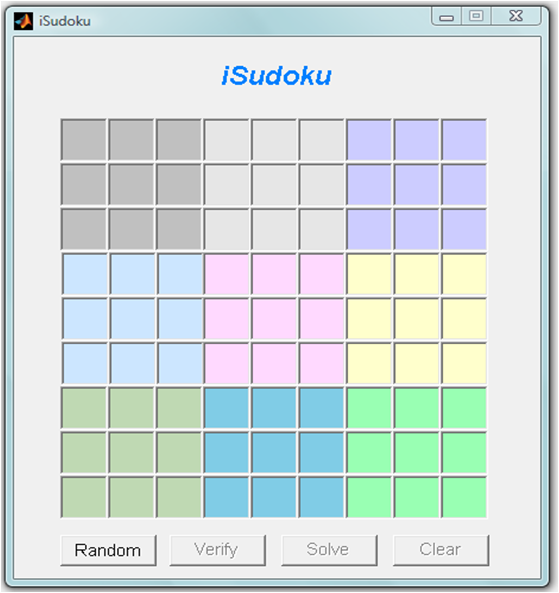
\includegraphics[scale = 0.7]{pictures/board1}
\caption{Sudoku GUI at initial state}
\label{fig:board1}
\end{figure}
\newline
\\The Sudoku board is represented by 81 textboxes, where each 3 by 3 sub square uses a different background color in order to be distinguished from each other.  Moreover, four push buttons are used to achieve the program’s functionality. These buttons are called random, solve, verify and clear. Figure \ref{fig:board1} illustrates the Sudoku’s GUI at its initial state.
\newline
\\The random button creates and displays a random game on the board. This is done by selecting a game from a database of several games. This button is the only one enabled when the application is started. Once a game has been displayed, the remaining buttons get enabled and only the empty cells can be edited. This means, that the hint cells cannot be modified by the user. An example of a random game is depicted at Figure \ref{fig:board2}, where its hint cells are displayed in black.
\begin{figure}[h!]
\centering
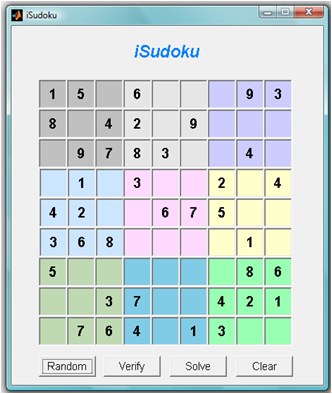
\includegraphics[scale = 1.4]{pictures/board2}
\caption{A random game and its hint cells}
\label{fig:board2}
\end{figure}
\newline
\\The solve button solves the current game and displays the solution on the board. This is achieved in three main steps:
\begin{enumerate}
\item Read the current game from the board and generate a numerical matrix of 81 elements, where the empty cells are substituted by zeros. A validation of the input data is performed in order to avoid sending invalid values to the algorithm. Only integer values from one to nine can be inserted in the cells. 
\item Execute the Sudoku solver function, \textit{iSudokuALG}, using the numerical matrix as an input.
\item Retrieve the solution provided by the Sudoku solver function and populate the board. The hint cells remain in black while the solution cells are highlighted in red. Figure \ref{fig:board3} depicts a solution of a game.
\end{enumerate}
\begin{figure}[h!]
\centering
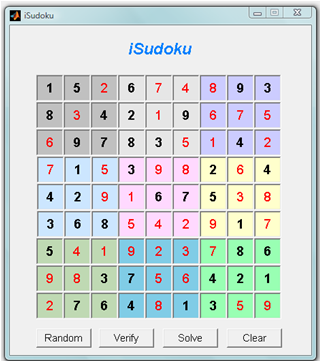
\includegraphics[scale = 1.4]{pictures/board3}
\caption{A solved game}
\label{fig:board3}
\end{figure}
The verify button examines the correctness of either a partial game or a complete game. If a partial or a complete game is detected to be incorrect, the program will display a pop-up window with an error message.  Otherwise, a different pop-up window will display a message stating that the game is correct and in case of a partial game, the message will also state the number of remaining empty cells. An example of these type of messages is illustrated at Figure \ref{fig:msgCorrect} and Figure \ref{fig:msgIncorrect}
\begin{figure}[ht!]
\label{fig:msgBox}
\begin{center}
%
\subfigure[Correct Game]{%
\label{fig:msgCorrect}
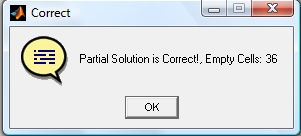
\includegraphics[width=0.52\textwidth]{pictures/Popup1}
}%
\subfigure[Incorrect Game]{%
\label{fig:msgIncorrect}
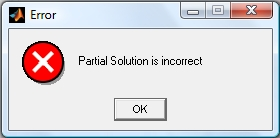
\includegraphics[width=0.49\textwidth]{pictures/Popup2}
}
\end{center}
\caption{%
GUI Message Boxes
}%
\end{figure}
\newline
\\Finally, the clear button implements the simplest functionality as it only clears the board and disables all the buttons except the random one, returning the program to its initial state.
\subsubsection{Game Database}
In order to have different games to be solved by the program an Excel database was created. This database includes games of different levels of difficulty, which means that the number of hints varies from game to game. All the games are contained within an Excel worksheet that is read when the GUI is initialized. An extract of the game database can be seen at Figure \ref{fig:excel}.
\begin{figure}[h!]
\centering
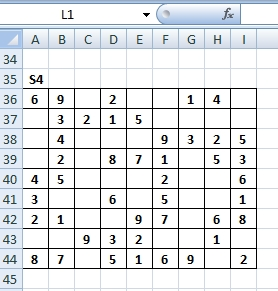
\includegraphics[scale = 0.6]{pictures/Excel1}
\caption{Extract of the Excel game database}
\label{fig:excel}
\end{figure}
\newline
\\The reading process is performed by means of MATLAB’s built-in function \textit{xlsread}. This function receives as input the name of the Excel file and the worksheet to be read. The output of this function is stored into a cell matrix that later on is used by the random button to select a game. This function is represented by the following:
\begin{verbatim}
% Read predefined games from the input spreadsheet
[num, cellMat]= xlsread('sudoku.xls', 'Games');
\end{verbatim}
%--------------------------GUI end-----------------------------------
\newpage
\subsection{An Algorithm for Solving Sudoku Puzzles}
The algorithm was implemented in MATLAB using direct puzzle search and constraint propagation. The constraint propagation was implemented in such a manner that: 
\begin{itemize}
\item When a value is assigned to a square that same value cannot be used as a possible assignment in all related cells;
\item If a cell has only one single value for possible assignment, that value is immediately assigned.
\end{itemize}
Our MATLAB program has only 4 steps:
\begin{enumerate}
\item Find all the possible values for all empty cells;
\item If there is a single possible value, we assign that value to the cell;
\item Propagate constraints to other cells;
\item If all the cells have more than one possible value we fill in a tentative value for that cell.
\end{enumerate}
This algorithm, though it is simplistic, it should perform fairly well  because of the algorithm's nature, as described in \cite{norvigsolving}. The process is performed by $iSudokuALG$ function. This function receives as an input parameter the cell matrix $A$ and gives as output a solved puzzle in the form of a matrix. This is represented by
\begin{verbatim}
% Read predefined games and outputs the solved puzzle
function [A]= iSudokuALG(A)
\end{verbatim}
Also we have implemented a function in order to perform a correctness verification function. This function has as input the cell matrix $A$ which contains the current puzzle. The output of the function is stored in variable $val$ which can have two values: $0$ if the puzzle is correct and $1$ otherwise. We represented the verification function as
\begin{verbatim}
% Puzzle verification function
function [val]=verific(A)
\end{verbatim}
To see how our program works, we will use a simpler 4-by-4 grid with 2-by-2 blocks. As mentioned in \cite{crook2009pencil} these kinds of puzzles are called Shidoku ("Shi" means "four" in Japanese). 
\begin{figure}[ht!]
\label{fig:subfigures}
\begin{center}
%
\subfigure[A Shidoku puzzle]{%
\label{fig:first}
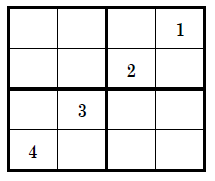
\includegraphics[width=0.4\textwidth]{pictures/1.png}
}%
\subfigure[The possible candidates for all squares]{%
\label{fig:second}
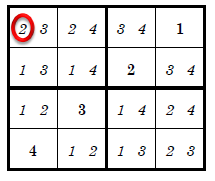
\includegraphics[width=0.4\textwidth]{pictures/2.png}
}\\ % ------- End of the first row ----------------------%
\subfigure[Inserting value 2 and constraint propagation]{%
\label{fig:third}
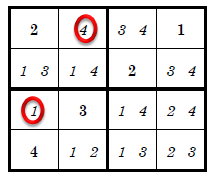
\includegraphics[width=0.4\textwidth]{pictures/3.png}
}%
\subfigure[Constraint propagation]{%
\label{fig:fourth}
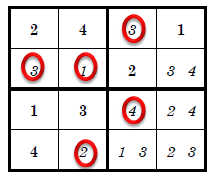
\includegraphics[width=0.4\textwidth]{pictures/4.png}
}\\ % ------- End of the second row ----------------------%
\subfigure[Insert the remaining values to complete the puzzle]{%
\label{fig:fifth}
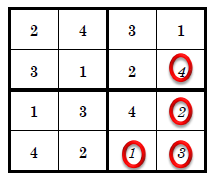
\includegraphics[width=0.4\textwidth]{pictures/5.png}
}%
\subfigure[The puzzle completed]{%
\label{fig:sixth}
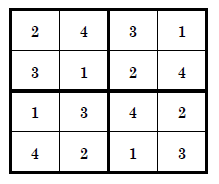
\includegraphics[width=0.4\textwidth]{pictures/6.png}
}
\end{center}
\caption{%
The algorithm for solving a simple Shidoku puzzle 
}%
\end{figure}
Figure \ref{fig:first} shows a Shidoku puzzle. Figure \ref{fig:second} through Figure \ref{fig:sixth} shows how we get to a solution by using our algorithm. In Figure \ref{fig:second}, the possible assignment, are represented as smaller digits. Also for example in Figure \ref{fig:second} line 1, row 1, we show that we have two possible values to choose from. If a cell contains only one candidate it is filled immediately.
\newline
\section{Experimental Results}
In this section we are presenting some experimental results using different input puzzles and we will describe how our MATLAB implementation behaves to various situations.
\subsection{User Interface Testing}
After developing the user interface, the functionality associated to each GUI component was tested. More specifically, it was verified the absence of run-time errors shown in MATLAB’s command window when the user executes an action. For example, when launching the application or when clicking any of the available buttons, no errors are displayed. Additionally, the program flow was tested to ensure that multiple Sudoku games can be solved without closing and opening the application when a game is finished.
\newline
\\In order to verify the correct operation of the \textit{random} and \textit{solve} buttons, it was checked that all of the Sudoku games in the database could be randomly selected and solved correctly. Similarly, the \textit{verify} button was tested by manually entering incorrect numbers and characters in the Sudoku board. The purpose of this test was to verify that the pop-up error messages are displayed when the proposed solution is incorrect. Finally, the \textit{clear} button was verified by checking that all of the cells in the board are cleared when the button is pushed.
\newline
\\The only issue found during the verification phase for the GUI was related to MATLAB’s xlsread function when using Microsoft Excel 2010. Apparently this is a well documented problem \footnote{http://www.mathworks.com/matlabcentral/newsreader/view\_thread/287717\#766161} regarding how the latest version of Excel handles COM objects and activeX commands which are used by this function . Nevertheless, the xlsread function works correctly when using previous versions of Excel, like version 2007. 
\subsection{Algorithm Testing}
All the algorithm source code was compiled and build using Matlab R2007a and is available online\footnote{http://goo.gl/96pCS}. The test system was a HP G7035EA laptop with 1.86 GHz Celeron Processor, 1 GB RAM and Windows XP as operating system.
\newline
\\ In order to verify and test our algorithm we have defined some test parameters. This parameters are $t_e$ (algorithm's execution time in seconds), $sq_{empty}$ (number of empty cells in a puzzle) and $s_i$ (steps or iterations done by the algorithm, meaning that one iteration starts when the solver begins the puzzle from the first cell and finishes when the last cell is computed). 
\begin{figure}[h!]
\centering
\includegraphics[scale = 0.37]{pictures/ts.jpg}
\caption{Experimental results for different Sudoku puzzles}
\label{fig:ts}
\end{figure}
Figure \ref{fig:ts} shows the results of our experiments for different $sq_{empty}$ in relation to $t_e$. We can say that $t_e$ is fluctuating in the interval $[0.06, 0.62]$ and $sq_{empty}$ for every puzzle is not a predictable measure of performance related to $t_e$. Also our algorithm is solving Sudoku puzzles with 40 empty cells in average and $s_i$ is varying between 2 and 9. After analysing all our results we can say that for relatively easy Sudoku puzzles our algorithm is performing quite well. 
\section{Conclusions}
Implementing a Sudoku solver in MATLAB allowed us to use many of the tools and built-in functions presented during the Numerical Methods course. For example, the utilization of loops, if-else statements and the manipulation of matrices and vectors. Nonetheless, we also learnt new functions by ourselves in order to enhance the application. For instance, we learnt to design GUIs, use pop-up windows to display messages and also importing data from Excel.
\newline
\\Nowadays, there are extensive studies regarding the mathematics of Sudoku as well as many different algorithms to solve the puzzles. Some algorithms are designed to solve the puzzles as quick as possible while some others are designed to solve them as efficiently in terms of computational power and memory. However, finding a suitable algorithm to solve any particular Sudoku game proved to be difficult.
\newline
\\The combination of a simple, yet effective algorithm with a graphical user interface allowed us to generate games, solve them and verify the given solutions in a simple and quick way. Additionally, the good communication and coordination among the team members made possible the completion of the project before the established deadline.

\bibliography{mybib}{}
\bibliographystyle{plain}
\end{document}

